\documentclass[a4paper,11pt,oneside]{article}

\usepackage[english]{babel}
\usepackage[utf8]{inputenc} 
\usepackage{graphicx}
\usepackage{subcaption}
\usepackage{caption}
\usepackage{verbatim}
\usepackage{amsmath,mathtools}
\usepackage[colorlinks,bookmarks=false,linkcolor=blue,urlcolor=blue]{hyperref}
\usepackage{booktabs}
\usepackage{hyperref}
\usepackage{listings}
\usepackage{color}
\usepackage{amssymb}
\usepackage{algorithm}
\usepackage[]{algpseudocode}
\usepackage{stackengine}
\usepackage[table,xcdraw]{xcolor}
\usepackage{pdfpages}
\usepackage{blindtext}
\usepackage{todonotes}
\usepackage[headsepline=1pt]{scrlayer-scrpage}
\usepackage[left=3cm,right=3cm,top=3cm,bottom=3cm]{geometry}
\usepackage{setspace}

%\newcommand{\HRule}{\rule{\linewidth}{0.5mm}}
\newcommand{\mail}[1]{{\href{mailto:#1}{#1}}}
\newcommand{\ftplink}[1]{{\href{ftp://#1}{#1}}}
\setstretch{1.3}


%\pagestyle{fancy}
%\fancyfoot[C]{\thepage}

\title{\textbf{Network Tour of DataScience}:\\ \normalfont Free Music Alternative Playlists}
\author{A. Buchegger \& L. Biotto \& J. Tapparel \& T. Tuuva}
\date{}


\automark{section}
\automark*{subsection}
\clearpairofpagestyles
\ihead{\headmark}
 


\begin{document}
\lstset{language=Matlab,%
    %basicstyle=\color{red},
    breaklines=true,%
    morekeywords={matlab2tikz},
    keywordstyle=\color{blue},%
    morekeywords=[2]{1}, keywordstyle=[2]{\color{black}},
    identifierstyle=\color{black},%
    stringstyle=\color{purple},
    commentstyle=\color{ForestGreen},%
    showstringspaces=false,%without this there will be a symbol in the places where there is a space
    numbers=left,%
    numberstyle={\tiny \color{black}},% size of the numbers
    numbersep=9pt, % this defines how far the numbers are from the text
    emph=[1]{for,end,break},emphstyle=[1]\color{red}, %some words to emphasise
    %emph=[2]{word1,word2}, emphstyle=[2]{style},
    frame = single,  
}
\maketitle

%\newpage
\section{Introduction}

It can be tough to know what we would like to listen when faced with an archive of thousand of musics. For our project we wondered how we could automatically generate a list of songs that would correspond to one's taste. We will explore the features of the Free Music Archive (FMA) to generate a graph that will contain many songs of selected genres. These songs can then be sorted and a playlist be generated out of a region of this graph. We will explore different methods of generating playlists. At the end, 
we will show how this tool can be used to generate a free alternative playlists from non-free musics.

\section{Generating the graph}
Thanks to Free Music Archive, we have access to a dataset of music from which we have a list of extracted features. In order to construct a graph from this song list, we considered each song as a node and calculated the euclidean distance between each node in the features space. We can then use these distances to define the weights of the edges between each nodes using the following formula:
$$
\text{Edge}_{\text{weight}}=e^{-\text{dist}^2/\text{dist}_{\text{mean}}^2}
$$
This would give us a strongly connected graph which would be long to process due to the high number of edges and having weakly weighted edges doesn't give very useful informations about the data structure. We can solve this problem by defining a minimal weight to keep an edge in the graph. One issue in doing that is the apparition of multiple components in the graph. For the future usage of this graph, we need it to be connected and to ensure that, we will only take into account the principal connected component and drop the nodes that aren't in it. In our implementation, we set the threshold value in order ensure that around 90\% of the nodes are in the main component.\\

Finally we place each node in a bi-dimensional space using a spring layout. This means that each node tries to get as far away from the others as it can, while being held back by the edges which are assimilated to springs, having a spring constant related to their corresponding weight.\\

Since processing the graph and placing the nodes in a 2D space requires an important amount of time, we limited the dataset to three balanced genres. The result of the created graph is presented on the figure \ref{fig:spring_layout}. However, these parameters can be chosen by the user at the moment he creates his own graph depending of his time and resources.

\begin{figure}[H]
\centering
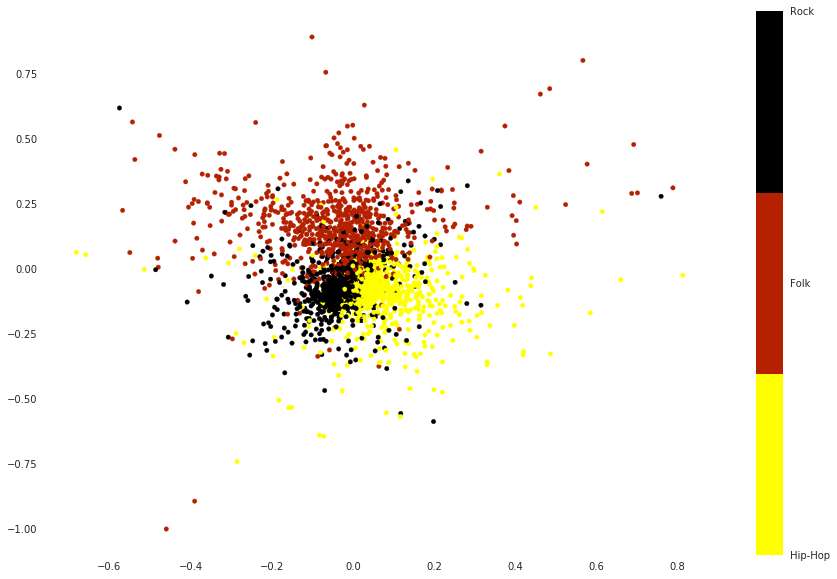
\includegraphics[width=\linewidth] {figures/graph_2}
\caption{Spring layout coloured by genre}
\label{fig:spring_layout}
\end{figure}
\section{Including our own songs}

To include our own music into the graph we first need to extract its features, this is done by using
the provided \textit{features.py} script(TODO REF). There are 518 features in total.
Then we can include the song in two ways:
\begin{itemize}
\item Recomputing the graph adjacency matrix with the new songs included.
\item Creating a KD-Tree of the graph, then searching for the nearest points in the K-features space for the included songs
\end{itemize}

\subsection{Inclusion by recomputation}
After having added the songs and their extracted features to the dataset, we simply generate a new graph in the same way. As expected it is a very time consuming method, getting worse as the dataset grows bigger. This led us to the next method. 

\subsection{Inclusion by nearest neighbour search}
Instead of recomputing the adjacency matrix and the corresponding graph, both having a high computational cost, we can estimate the new nodes position. To do so, we generate another kind of graph directly from the features, in our case we chose a KD-Tree.
An example of a 2D-Tree is presented in the figure~(\ref{fig:ex_tree})

This kind of structure is conceived to quickly find the nearest neighbours in an efficient way.
We decided to consider that the closest neighbour to our newly included song, in the features space, is going to be assimilated to the new node. Hence, when we want to extract a playlist, this existing node will be used. %TODO

\begin{figure}[H]
  \centering
    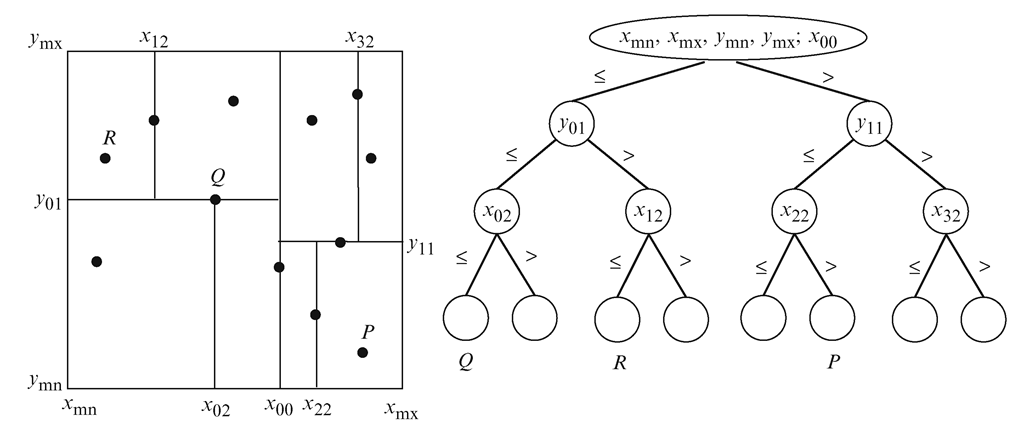
\includegraphics[width=\textwidth]{./Figures/tree}
  \caption{Example of a 2D-Tree}
  \label{fig:ex_tree}
\end{figure}

\section{Generating the playlist}

To generate a playlist we explored three distinct methods:
\begin{itemize}
\item Nearest neighbours in the features space
\item Nearest neighbours in the 2D-space of the spring layout graph 
\item Hottest nodes from a heat diffusion in the graph
\end{itemize}

\subsection{518D features exploration}
First, we can create a playlist directly from the euclidean distance between features. This property should result in similar features, such as rythm, or height of voice of example, but being more adventurous in regards to genres. One could for example end up listening to hip-hop when starting from rock.

\subsection{2D graph exploration}
Secondly, we select the closest songs around the selected music (node) in the graph. This effectively results in a kind of circle around a point. This type of playlist will thus be very targeted towards a specific kind of song. For this purpose we use the simple euclidean distance in our 2D graph.

\subsection{Graph heat diffusion}
Finally, we generate a heat diffusion around selected nodes, and create a playlist from the "warmest" nodes. To simulate this heat diffusion in the graph, we use the functions of PyGSP allowing us to generate the heat kernel filter and apply it to our graph. We provide a graph in node domain but the filtering is performed in frequency domain.\\

With this method it is possible to mix the diffusion from each starting node which result to a playlist being between every given song. For example, if we give a rock song and a rap song, we will get some songs which are fusions of rock and rap.

This selection should result in a kind of path between different closely connected songs.When listening to a playlist, it is nice to be able to tell how adventurous we feel regarding the inclusion of other styles. Therefore we let the user choose the heat diffusion parameter "tau". 

\begin{figure}[H]
  \centering
    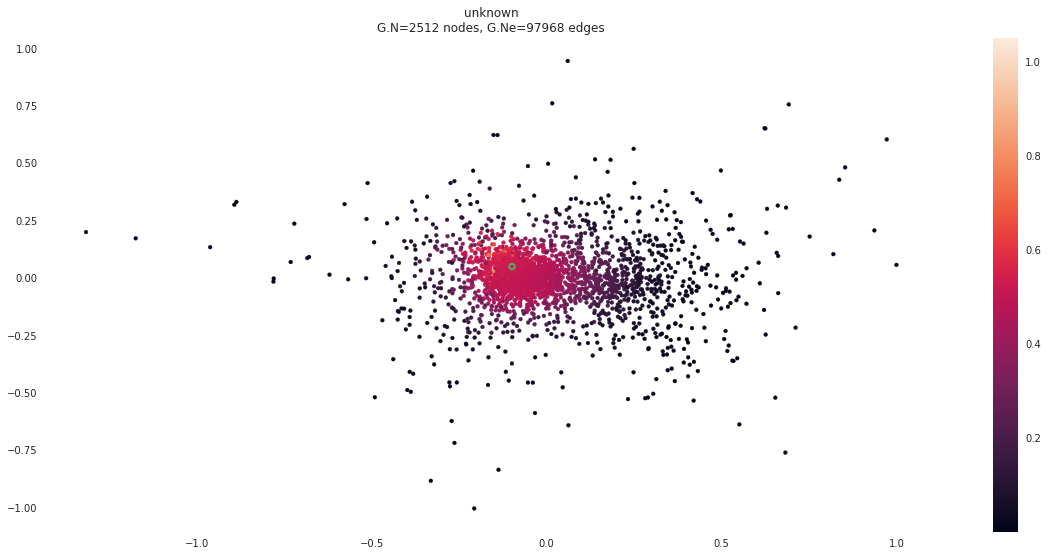
\includegraphics[width=\textwidth]{./Figures/heat}
  \caption{Heat spreading starting from one node(green marker)}
  \label{fig:}
\end{figure}

\newpage
\section{Conclusion}




\end{document}
